\documentclass[11pt,a4paper,ngerman]{article}
\usepackage[bottom=2.5cm,top=2.5cm]{geometry} 
\usepackage{babel}
\usepackage[utf8]{inputenc} 
\usepackage[T1]{fontenc} 
\usepackage{ae} 
\usepackage{amssymb} 
\usepackage{amsmath}
\usepackage{amsthm} 
\usepackage{graphicx}
\usepackage{fancyhdr}
\usepackage{caption}
\usepackage{subcaption}
\usepackage{fancyref}
\usepackage{enumerate}
\usepackage{listings}
\usepackage{xcolor}
\usepackage{paralist}
\usepackage{tabularx}

\usepackage[pdftex, bookmarks=false, pdfstartview={FitH}, linkbordercolor=white]{hyperref}
\usepackage{fancyhdr}
\pagestyle{fancy}
\fancyhead[C]{Numerik I}
\fancyhead[L]{Übung 8}
\fancyhead[R]{SoSe 2013}
\fancyfoot{}
\fancyfoot[L]{}
\fancyfoot[C]{\thepage \hspace{1px} of \pageref{LastPage}}
\renewcommand{\footrulewidth}{0.5pt}
\renewcommand{\headrulewidth}{0.5pt}
\setlength{\parindent}{0pt} 
\setlength{\headheight}{0pt}

\date{Tutor: Christina Schulz}
\title{Übung 8}
\author{Max Wisniewski, Alexander Steen}


%%
%% Enviroments for proofs and lemmas
%%
\newtheorem{lemma}{\bfseries Claim}

\begin{document}

\lstset{language=Pascal, basicstyle=\ttfamily\fontsize{10pt}{10pt}\selectfont\upshape, commentstyle=\rmfamily\slshape, keywordstyle=\rmfamily\bfseries, breaklines=true, frame=single, xleftmargin=3mm, xrightmargin=3mm, tabsize=2, mathescape=true}

\renewcommand{\figurename}{Figure}

\maketitle
\thispagestyle{fancy}

%%%%%%%%%%%%%%%%%%%%%%%%%%%%%%
%% Aufgabe 1     %%%%%%%%%%%%%%%%
%%%%%%%%%%%%%%%%%%%%%%%%%%%%%%
\subsection*{Aufgabe 1}
Das Listing~\ref{alg:romberg} zeigt unsere Implementierung der klassichen Romberg-Quadratur.
Bei Eingabe der Integrationsgrenzen, der Funktion und der Liste von Gitterbreiten, wird (wie 
im Skript gezeigt) nach dem Aitken-Neville-Schema die Extrapolation berechnet.
Der Aufruf von \texttt{trapQuad} in der Funktion ist eine leicht modifizierte Version der Funktion vom letzten Übungszettel. Hier wird nicht mehr die Gitterbreite und der Start- und Endpunkt übergeben, sondern das Gittern selber (macht den Code kürzer).

\begin{lstlisting}[language=matlab, numbers=left, caption=Klassische Romberg-Quadratur, label=alg:romberg]
function [S] = romberg(a,b,f,h)
% Gibt den Zahlenwert S der klassischen
% Romberg-Quadratur zurueck
%
% [a,b] Integrationsintervall
% f zu intigrierende Funktion
% h Liste der Schrittweiten
%  (absteigende Gitterbreite!)

% Anzahl der Gitterbreiten
n = length(h);

t = zeros(n,1);

%% Berechnung nach Aitken-Neville-Schema
%% mit Rekursion aus dem Skript
for i = 1:n
  %% summierte Trapezregel zur breite h_i
  t(i) = trapQuad(a:h(i):b,f);
  %% Rekursion
  for k = i:-1:1
    t(k) = t(k+1) + (t(k+1)-t(k))/((h(k)/h(i))^2 - 1);
  end
end
S = t(1);
\end{lstlisting}

Der Test der Funktion wurde wie folgt durchgeführt (Kommentare im Listing).

\begin{lstlisting}[language=matlab,numbers=left]
%% f1 und f2 sind die beiden zu integrierenden Funktionen
f1 = @(x) 1/(2*atan(1)) * 1/(1+x^2);
f2 = @(x) 1/(2*atan(500)) * 1/(1+(500*x)^2);
%% 12x2 Matrizen zur Speicherung der Ergebnisse
%% beider Methoden bei Eingabe f1 bzw. f2
rombergQuad = zeros(12,2);
trapezQuad = zeros(12,2);
%% 12x2 Matrizen der absoluten Fehler
%% beider Methoden
fehlerRomberg = zeros(12,2);
fehlerTrapez = zeros(12,2);
%% Berechnung der Quadratur und Fehler
for i = 1:12
  trapezQuad(i,1) = trapQuad(-1:2^(-i):1,f1);
  trapezQuad(i,2) = trapQuad(-1:2^(-i):1,f2);
  rombergQuad(i,1) = romberg(-1,1,f1,2.^(-[0:i]));
  rombergQuad(i,2) = romberg(-1,1,f2,2.^(-[0:i]));
  fehlerTrapez(i,1) = abs(trapezQuad(i,1) - 1);
  fehlerTrapez(i,2) = abs(trapezQuad(i,2) - 1);
  fehlerRomberg(i,1) = abs(rombergQuad(i,1) - 1);
  fehlerRomberg(i,2) = abs(rombergQuad(i,2) - 1);
end
\end{lstlisting}

Es ergeben sich folgende Fehler (die linke Spalte sind die Fehler von \texttt{f1} ($\gamma = 1$), die rechte Spalte von \texttt{f2} ($\gamma = 500$)). In jeder Spalte ist die $i-te$ Zeile das Ergebnis der Quadratur mit
(feinstem) Gitter $h_i$, $i = 1,.., 12$.
\begin{lstlisting}[basicstyle=\ttfamily\scriptsize\selectfont\upshape]
fehlerTrapez =
   0.013239352830249   0.840636419672265
   0.003315574025695   0.920306878383561
   0.000828929586313   0.960129548066769
   0.000207232961173   0.980015760024551
   0.000051808249116   0.989908833068686
   0.000012952062417   0.994757042698583
   0.000003238015606   0.996997544736434
   0.000000809503901   0.997832792863140
   0.000000202375976   0.997993557291557
   0.000000050593994   0.997999989669726
   0.000000012648499   0.998000000000075
   0.000000003162123   0.998000000000025

fehlerRomberg =
   0.002629023290789   0.893754213535242
   0.000167110611374   0.950404330248577
   0.000002186734143   0.975566264743692
   0.000000003720382   0.987770983969616
   0.000000000015422   0.993770542341976
   0.000000000000023   0.996645736088292
   0.000000000000001   0.997862028038352
   0.000000000000001   0.998141905293127
   0.000000000000001   0.998040882362203
   0.000000000000000   0.997998214562390
   0.000000000000001   0.997999880717347
   0.000000000000002   0.998000002633203
\end{lstlisting}

Der Fehler beider Methoden bei Eingabe von $f$ mit $\gamma = 1$ wird schnell klein; bei der Romberg-Quadratur etwas schneller als bei der summierten Trapezregel. Bei Eingabe von $f$ mit $\gamma = 500$ wird bei beiden Verfahren der Fehler nicht kleiner, sondern sogar größer. Bei beiden Verfahren ist bei $n=12$ nazezu ein relativer Fehler von hundert Prozent zu beobachten. Es fällt auf, dass der Fehler der Romberg-Quadratur sogar schneller wächst als bei der summierten Trapezregel.

\begin{figure}[h!]
\centering
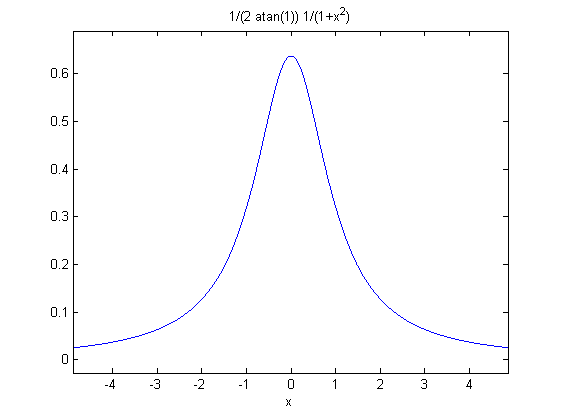
\includegraphics[width=0.48\textwidth]{f1.png}
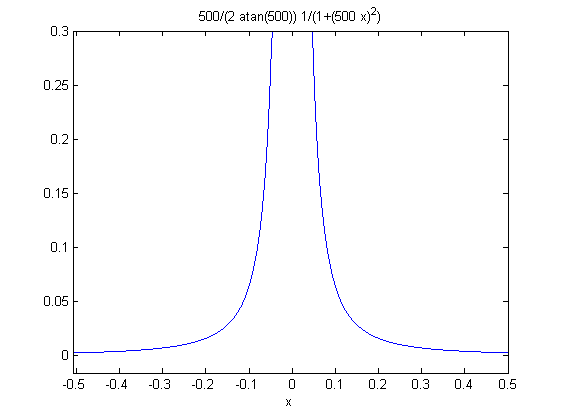
\includegraphics[width=0.48\textwidth]{f2.png}
\caption{Graph der Funktion $f$ mit $\gamma = 1$ (links) und $\gamma = 500$ (rechts) \label{fig:f}}
\end{figure}

Schaut man sich die Graphen der beiden Funktionen an (siehe Abbildung~\ref{fig:f}), so fällt auf, dass die erste Funktion sehr glatt ist, die zweite Funktionen eine (betragsmäßig) extrem große Steigung um 0 herum aufweist. Der Funktionswert an Stelle 0 fällt zu beiden seiten extrem schnell ab. Aus diesem Grund werden beide Quadraturen sehr ungenau, da die ''kleine Spitze'' des Graphen nicht korrekt berücksichtigt wird.

%%%%%%%%%%%%%%%%%%%%%%%%%%%%%%
%% Aufgabe 2     %%%%%%%%%%%%%%%%
%%%%%%%%%%%%%%%%%%%%%%%%%%%%%%
\subsection*{Aufgabe 2}


\label{LastPage}
\end{document}
